\documentclass[../main.tex]{subfiles}
\begin{document}
\section{Distributions after the baseline selection}
\label{hh:sec:control_plots}

The distributions of some of the main variables after the baseline categorization are shown in Fig.~\ref{hh:fig:control_mutau}, \ref{hh:fig:control_etau}, \ref{hh:fig:control_tautau}, and \ref{hh:fig:control_masses}, for the data and backgrounds in 2018. All corrections described in Section~\ref{hh:sec:corrections} are applied to simulated events. In all distributions there is a good agreement (in general within the statistical uncertainty range) between data and the expected backgrounds.





\begin{figure}[p!]
\begin{center}
\subfloat[$\mu$ $p_T$]{\includegraphics[width=0.333\textwidth]{Images/controlplots/baseline/lep1_pt__mutau_os_iso__qcd__stack}}
\subfloat[First b jet $p_T$]{\includegraphics[width=0.333\textwidth]{Images/controlplots/baseline/bjet1_pt__mutau_os_iso__qcd__stack}}
\subfloat[First VBF jet $p_T$]{\includegraphics[width=0.333\textwidth]{Images/controlplots/baseline/vbfjet1_pt__mutau_os_iso__qcd__stack}}\\
\subfloat[\tauh{} $p_T$]{\includegraphics[width=0.333\textwidth]{Images/controlplots/baseline/lep2_pt__mutau_os_iso__qcd__stack}}
\subfloat[Second b jet $p_T$]{\includegraphics[width=0.333\textwidth]{Images/controlplots/baseline/bjet2_pt__mutau_os_iso__qcd__stack}}
\subfloat[Second VBF jet $p_T$]{\includegraphics[width=0.333\textwidth]{Images/controlplots/baseline/vbfjet2_pt__mutau_os_iso__qcd__stack}}\\
\subfloat[$\mu$ $\eta$]{\includegraphics[width=0.333\textwidth]{Images/controlplots/baseline/lep1_eta__mutau_os_iso__qcd__stack}}
\subfloat[First b jet $\eta$]{\includegraphics[width=0.333\textwidth]{Images/controlplots/baseline/bjet1_eta__mutau_os_iso__qcd__stack}}
\subfloat[First VBF jet $\eta$]{\includegraphics[width=0.333\textwidth]{Images/controlplots/baseline/vbfjet1_eta__mutau_os_iso__qcd__stack}}\\
\subfloat[\tauh{} $\eta$]{\includegraphics[width=0.333\textwidth]{Images/controlplots/baseline/lep2_eta__mutau_os_iso__qcd__stack}}
\subfloat[Second b jet $\eta$]{\includegraphics[width=0.333\textwidth]{Images/controlplots/baseline/bjet2_eta__mutau_os_iso__qcd__stack}}
\subfloat[Second VBF jet $\eta$]{\includegraphics[width=0.333\textwidth]{Images/controlplots/baseline/vbfjet2_eta__mutau_os_iso__qcd__stack}}\\
\end{center}
\caption[Control plots for 2018, baseline category, and $\tau_\mu\tau_h$ channel]{Leptons and jets variable distributions in the baseline category, $\tau_\mu\tau_h$ channel, and 2018. The first b and VBF jet candidates out of the corresponding jet pairs are the ones with the highest $p_T$.}
\label{hh:fig:control_mutau}
\end{figure}


\begin{figure}[p!]
\begin{center}
\subfloat[e $p_T$]{\includegraphics[width=0.333\textwidth]{Images/controlplots/baseline/lep1_pt__etau_os_iso__qcd__stack}}
\subfloat[First b jet $p_T$]{\includegraphics[width=0.333\textwidth]{Images/controlplots/baseline/bjet1_pt__etau_os_iso__qcd__stack}}
\subfloat[First VBF jet $p_T$]{\includegraphics[width=0.333\textwidth]{Images/controlplots/baseline/vbfjet1_pt__etau_os_iso__qcd__stack}}\\
\subfloat[\tauh{} $p_T$]{\includegraphics[width=0.333\textwidth]{Images/controlplots/baseline/lep2_pt__etau_os_iso__qcd__stack}}
\subfloat[Second b jet $p_T$]{\includegraphics[width=0.333\textwidth]{Images/controlplots/baseline/bjet2_pt__etau_os_iso__qcd__stack}}
\subfloat[Second VBF jet $p_T$]{\includegraphics[width=0.333\textwidth]{Images/controlplots/baseline/vbfjet2_pt__etau_os_iso__qcd__stack}}\\
\subfloat[e $\eta$]{\includegraphics[width=0.333\textwidth]{Images/controlplots/baseline/lep1_eta__etau_os_iso__qcd__stack}}
\subfloat[First b jet $\eta$]{\includegraphics[width=0.333\textwidth]{Images/controlplots/baseline/bjet1_eta__etau_os_iso__qcd__stack}}
\subfloat[First VBF jet $\eta$]{\includegraphics[width=0.333\textwidth]{Images/controlplots/baseline/vbfjet1_eta__etau_os_iso__qcd__stack}}\\
\subfloat[\tauh{} $\eta$]{\includegraphics[width=0.333\textwidth]{Images/controlplots/baseline/lep2_eta__etau_os_iso__qcd__stack}}
\subfloat[Second b jet $\eta$]{\includegraphics[width=0.333\textwidth]{Images/controlplots/baseline/bjet2_eta__etau_os_iso__qcd__stack}}
\subfloat[Second VBF jet $\eta$]{\includegraphics[width=0.333\textwidth]{Images/controlplots/baseline/vbfjet2_eta__etau_os_iso__qcd__stack}}\\
\end{center}
\caption[Control plots for 2018, baseline category, and $\tau_e\tau_h$ channel]{Leptons and jets variable distributions in the baseline category, $\tau_e\tau_h$ channel, and 2018. b and VBF jet candidates are ordered by $p_T$.}
\label{hh:fig:control_etau}
\end{figure}



\begin{figure}[p!]
\begin{center}
\subfloat[First $\tau_{h}$ $p_T$]{\includegraphics[width=0.333\textwidth]{Images/controlplots/baseline/lep1_pt__tautau_os_iso__qcd__stack}}
\subfloat[First b jet $p_T$]{\includegraphics[width=0.333\textwidth]{Images/controlplots/baseline/bjet1_pt__tautau_os_iso__qcd__stack}}
\subfloat[First VBF jet $p_T$]{\includegraphics[width=0.333\textwidth]{Images/controlplots/baseline/vbfjet1_pt__tautau_os_iso__qcd__stack}}\\
\subfloat[Second \tauh{} $p_T$]{\includegraphics[width=0.333\textwidth]{Images/controlplots/baseline/lep2_pt__tautau_os_iso__qcd__stack}}
\subfloat[Second b jet $p_T$]{\includegraphics[width=0.333\textwidth]{Images/controlplots/baseline/bjet2_pt__tautau_os_iso__qcd__stack}}
\subfloat[Second VBF jet $p_T$]{\includegraphics[width=0.333\textwidth]{Images/controlplots/baseline/vbfjet2_pt__tautau_os_iso__qcd__stack}}\\
\subfloat[First $\tau_h$ $\eta$]{\includegraphics[width=0.333\textwidth]{Images/controlplots/baseline/lep1_eta__tautau_os_iso__qcd__stack}}
\subfloat[First b jet $\eta$]{\includegraphics[width=0.333\textwidth]{Images/controlplots/baseline/bjet1_eta__tautau_os_iso__qcd__stack}}
\subfloat[First VBF jet $\eta$]{\includegraphics[width=0.333\textwidth]{Images/controlplots/baseline/vbfjet1_eta__tautau_os_iso__qcd__stack}}\\
\subfloat[Second \tauh{} $\eta$]{\includegraphics[width=0.333\textwidth]{Images/controlplots/baseline/lep2_eta__tautau_os_iso__qcd__stack}}
\subfloat[Second b jet $\eta$]{\includegraphics[width=0.333\textwidth]{Images/controlplots/baseline/bjet2_eta__tautau_os_iso__qcd__stack}}
\subfloat[Second VBF jet $\eta$]{\includegraphics[width=0.333\textwidth]{Images/controlplots/baseline/vbfjet2_eta__tautau_os_iso__qcd__stack}}\\
\end{center}
\caption[Control plots for 2018, baseline category, and $\tau_h\tau_h$ channel]{Leptons and jets variable distributions in the baseline category, $\tau_h\tau_h$ channel, and 2018. First $\tau_h$ corresponds to the most isolated $\tau_h$ of the $\tau\tau$ pair, while b and VBF jet candidates are ordered by $p_T$.}
\label{hh:fig:control_tautau}
\end{figure}



\begin{figure}[p!]
\begin{center}
\subfloat[H($\tau\tau$) mass, $\tau_\mu\tau_h$ ch.]{\includegraphics[width=0.333\textwidth]{Images/controlplots/baseline/Htt_svfit_mass__mutau_os_iso__qcd__stack}}
\subfloat[H($\tau\tau$) mass, $\tau_e\tau_h$ ch.]{\includegraphics[width=0.333\textwidth]{Images/controlplots/baseline/Htt_svfit_mass__etau_os_iso__qcd__stack}}
\subfloat[H($\tau\tau$) mass, $\tau_h\tau_h$ ch.]{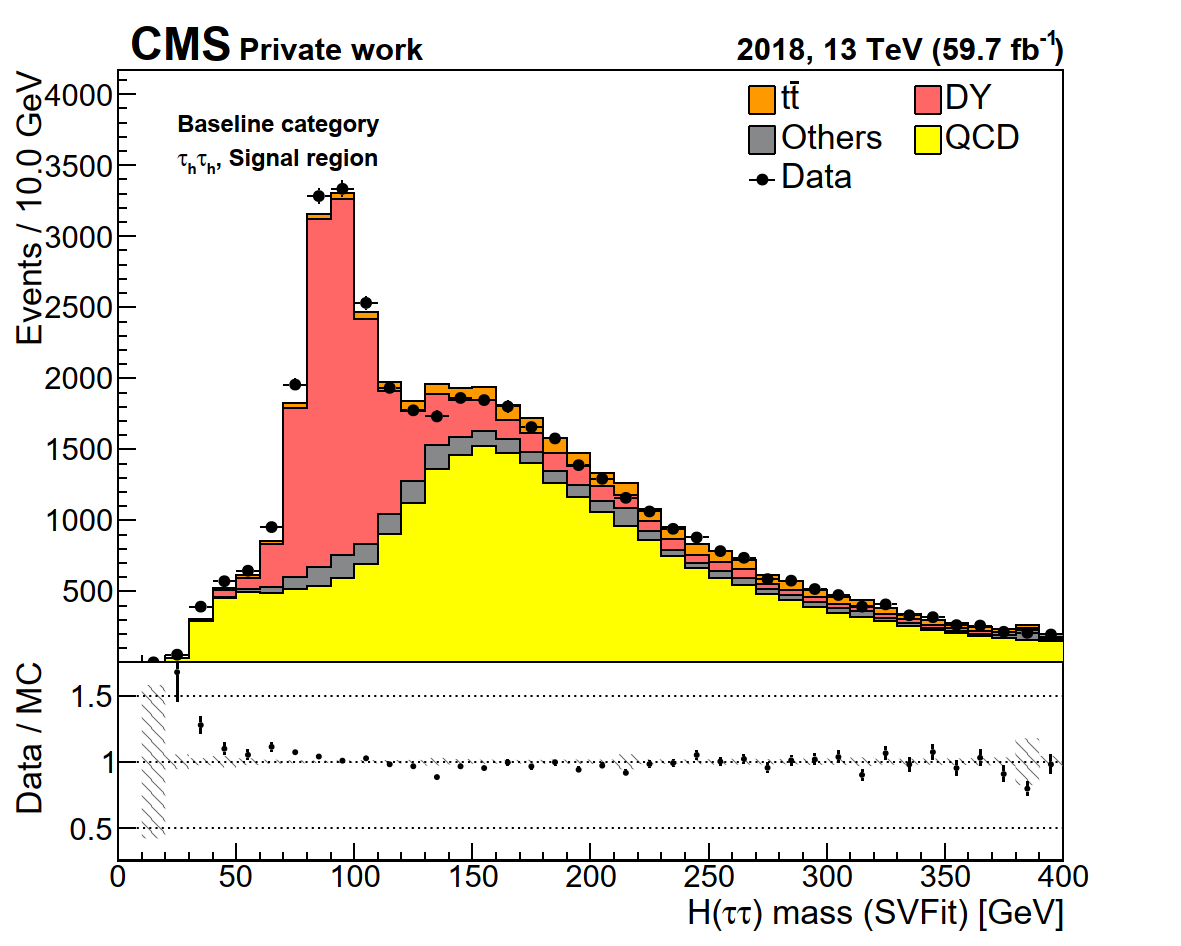
\includegraphics[width=0.333\textwidth]{Images/controlplots/baseline/Htt_svfit_mass__tautau_os_iso__qcd__stack}}\\
\subfloat[H(bb) mass, $\tau_\mu\tau_h$ ch.]{\includegraphics[width=0.333\textwidth]{Images/controlplots/baseline/Hbb_mass__mutau_os_iso__qcd__stack}}
\subfloat[H(bb) mass, $\tau_e\tau_h$ ch.]{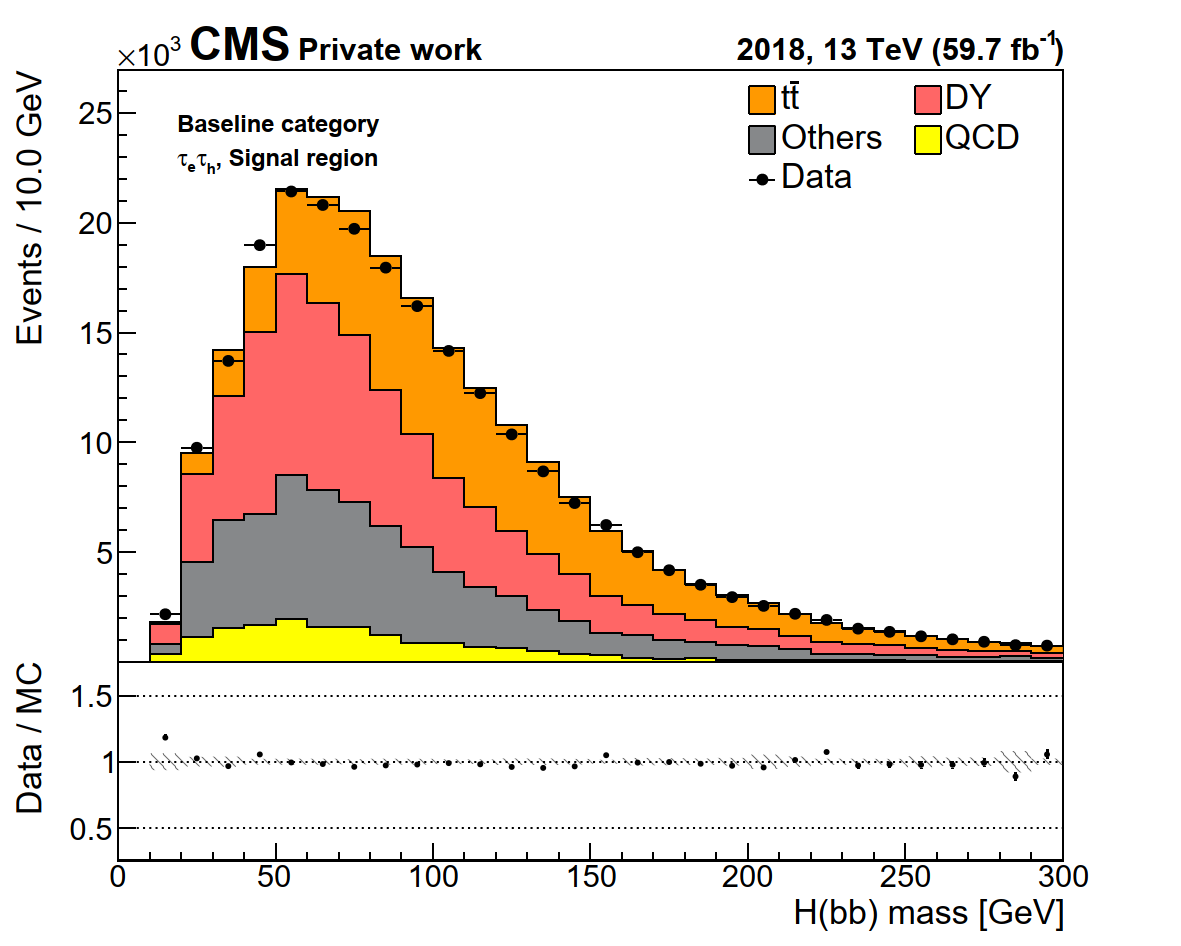
\includegraphics[width=0.333\textwidth]{Images/controlplots/baseline/Hbb_mass__etau_os_iso__qcd__stack}}
\subfloat[H(bb) mass, $\tau_h\tau_h$ ch.]{\includegraphics[width=0.333\textwidth]{Images/controlplots/baseline/Hbb_mass__tautau_os_iso__qcd__stack}}\\
\subfloat[HH mass, $\tau_\mu\tau_h$ ch.]{\includegraphics[width=0.333\textwidth]{Images/controlplots/baseline/Hbb_mass__mutau_os_iso__qcd__stack}}
\subfloat[HH mass, $\tau_e\tau_h$ ch.]{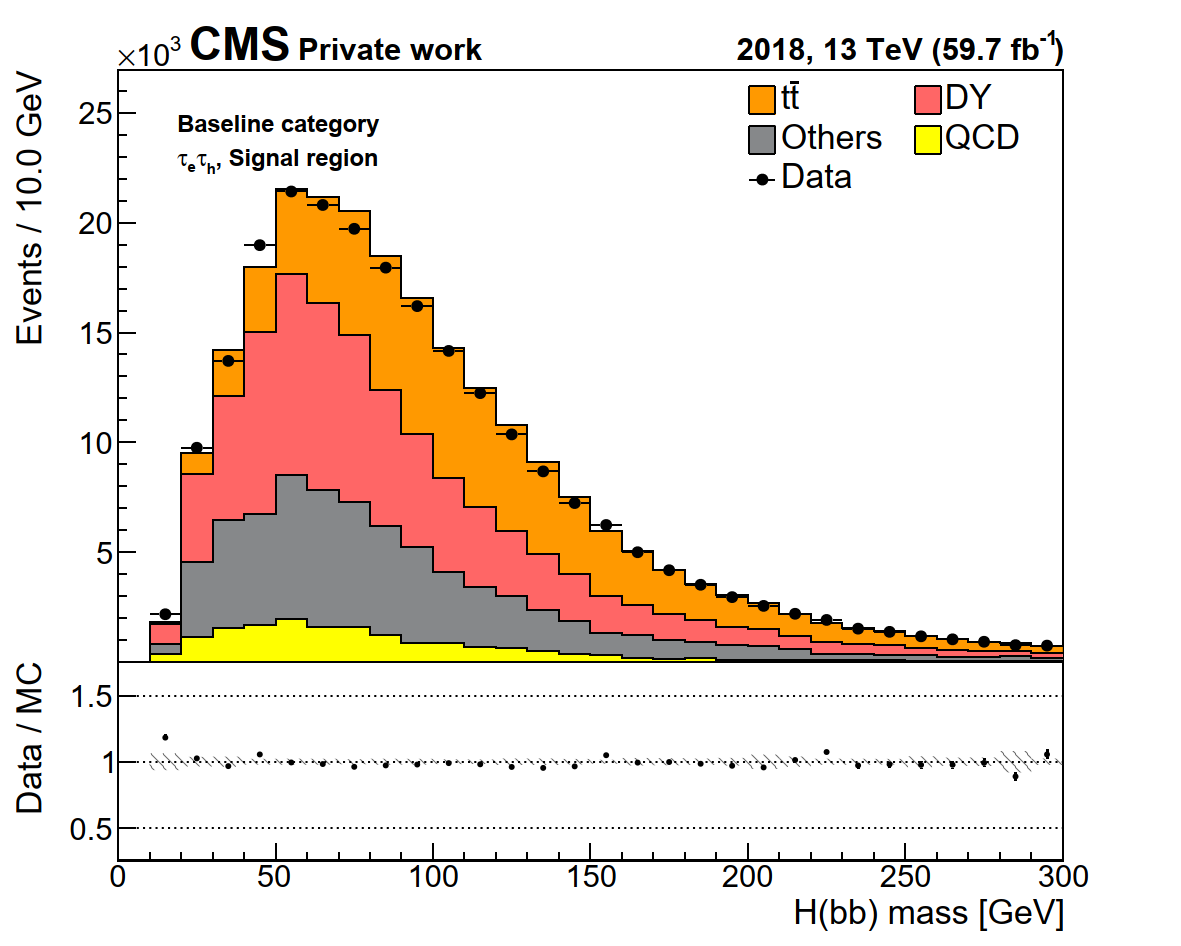
\includegraphics[width=0.333\textwidth]{Images/controlplots/baseline/Hbb_mass__etau_os_iso__qcd__stack}}
\subfloat[HH mass, $\tau_h\tau_h$ ch.]{\includegraphics[width=0.333\textwidth]{Images/controlplots/baseline/Hbb_mass__tautau_os_iso__qcd__stack}}\\
\subfloat[VBF ($j_1,j_2$) mass, $\tau_\mu\tau_h$ ch.]{\includegraphics[width=0.333\textwidth]{Images/controlplots/baseline/vbfjj_mass__mutau_os_iso__qcd__stack}}
\subfloat[VBF ($j_1,j_2$) mass, $\tau_e\tau_h$ ch.]{\includegraphics[width=0.333\textwidth]{Images/controlplots/baseline/vbfjj_mass__etau_os_iso__qcd__stack}}
\subfloat[VBF ($j_1,j_2$) mass, $\tau_h\tau_h$ ch.]{\includegraphics[width=0.333\textwidth]{Images/controlplots/baseline/vbfjj_mass__tautau_os_iso__qcd__stack}}\\
\end{center}
\caption[Mass control plots for 2018 and baseline category]{H($\tau\tau$), H(bb), HH, and VBF ($j_1,j_2$) system mass distributions in the baseline category, $\tau_\mu\tau_h$, $\tau_e\tau_h$, and $\tau_h\tau_h$ channels, in 2018.}
\label{hh:fig:control_masses}
\end{figure}



\end{document}

